\documentclass[12pt, twoside]{article}
\usepackage[letterpaper, margin=1in, head=30pt, headsep=0.1in]{geometry}
\usepackage[english]{babel}
\usepackage[utf8]{inputenc}
\usepackage{amsmath}
\usepackage{amsfonts}
\usepackage{amssymb}
\usepackage{tikz}
\usepackage{yhmath} %arcs using \wideparen{}
\usetikzlibrary{quotes, angles}

\usepackage{graphicx}
\usepackage{enumitem}
\usepackage{multicol}

%\usepackage{pgfplots}
%\pgfplotsset{width=10cm,compat=1.9}
%\usepgfplotslibrary{statistics}
%\usepackage{pgfplotstable}
%\usepackage{tkz-fct}
%\usepackage{venndiagram}

\usepackage{fancyhdr}
\pagestyle{fancy}
\fancyhf{}
\renewcommand{\headrulewidth}{0pt} % disable the underline of the header
\raggedbottom
\newif\ifmeta
\metatrue %print standards and topics tags

\title{High School Geometry problem sets}
\author{Chris Huson}
\date{April 2021}

%\fancyhead[RE]{\thepage}
%\fancyhead[RO]{\thepage \\ Name: \hspace{3cm}}
%\fancyhead[L]{BECA / Dr. Huson / 10th Grade Geometry\\* 7 June 2019}
%
%\begin{document}
%\subsubsection*{13.7 Homework: Cross sections, distance applications}
%\fancyhead[L]{BECA / Dr. Huson / Geometry 03-Volume+angle-bisectors\\* pset ID: 34}

\begin{document}

\subsubsection*{9.2 Tangent and slope}
\begin{enumerate}
\item Do Now: Given a triangle $\triangle ABC$ having angles with measures $m\angle A = 45^\circ$ and $m\angle C = 90^\circ$. Find the measure of the third angle, $m\angle B$.

\newpage
\item Do Now: Convert units of \emph{radians} and \emph{degrees} ($2 \pi = 360^\circ$, $\pi = 180^\circ$).\\[0.25cm]
  Apply the appropriate formula.
  \begin{multicols}{2}
    $\displaystyle d = r \times \frac{180}{\pi}$\\
    $\displaystyle r = d \times \frac{\pi}{180}$
  \end{multicols} \vspace{0.5cm}
  \begin{multicols}{2}
    \raggedcolumns
    \begin{enumerate}
      \item $\displaystyle m\angle A = \frac{\pi}{4}  =\hspace{0.15cm} ?$ degrees\\[0.75cm]
      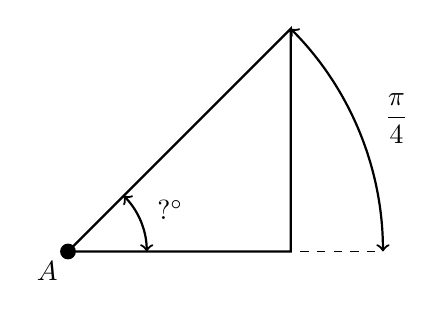
\begin{tikzpicture}[scale=1]
        \draw [thick, <->] (0:1) arc (0:45:1);
        \draw [thick, <->] (0:4) arc (0:45:4);
        \draw [dashed](0,0)--(4,0);
        \draw [thick]
        (0,0) node[below left] {$A$}--(45:4)--(2.83,0)--cycle;
        \fill (0,0) circle[radius=.1];
        \node at (22:1.4) {$?^\circ$};
        \node at (22:4.5) {$\displaystyle \frac{\pi}{4}$};
      \end{tikzpicture}
      \columnbreak
      \item $m\angle B = 30^\circ = \hspace{0.15cm} ?$ radians \\
      (in terms of $\pi$)\\[0.5cm]
      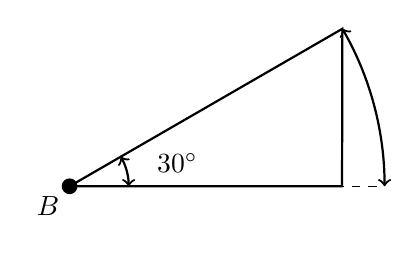
\begin{tikzpicture}[scale=1]
        \draw [thick, <->] (0:0.75) arc (0:30:0.75);
        \draw [thick, <->] (0:4) arc (0:30:4);
        \draw [dashed](0,0)--(4,0);
        \draw [thick]
        (0,0) node[below left] {$B$}--(30:4)--(3.46,0)--cycle;
        \fill (0,0) circle[radius=.1];
        \node at (12:1.4) {$30^\circ$};
      \end{tikzpicture}
    \end{enumerate}
  \end{multicols}

\newpage
\item Do Now: Write down the slope perpendicular to the given slope. (negative reciprocal) \vspace{0.5cm}
\begin{enumerate}
  \begin{multicols}{2}
  \item   $m= \frac{1}{3} \hspace{1cm} m_{\perp} = $
  \item   $m= -0.8 \hspace{1cm} m_{\perp} = $ 
  \end{multicols}
\end{enumerate}

\newpage
\item $\triangle ABC$ is shown with $m\angle C=90^\circ$ and the lengths of the triangle's sides are $BC=8$, $AC=15$, and $AB=17$. (not drawn to scale)
  \begin{multicols}{2}
    \begin{enumerate}
      \item How long is the \emph{hypotenuse}? \vspace{0.5cm}
      \item How long is the side \emph{opposite} $\angle A$? \vspace{0.5cm}
      \item How long is the side \emph{adjacent} to $\angle A$? \vspace{0.5cm}
    \end{enumerate}
    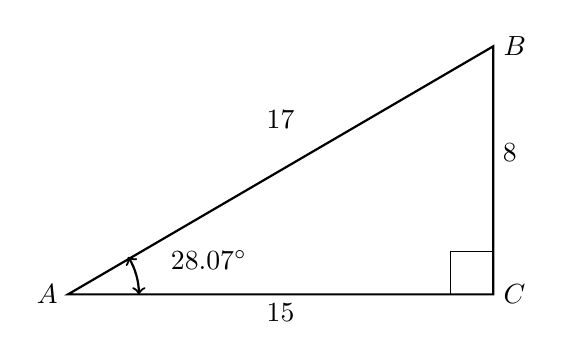
\begin{tikzpicture}[scale=0.9]
      \draw [thick]
      (0,0)node[left]{$A$}--
      (6,0)node[ right]{$C$}--
      (6,3.5)node[right]{$B$}--cycle;
      \draw (6,0)++(-0.6,0)--++(0,0.6)--+(0.6,0);
      \draw [thick, <->] (0:1) arc (0:32:1);
      \node at (20:1.4)[right]{$28.07^\circ$};
      \node at (3,0)[below]{$15$};
      \node at (6,2)[right]{$8$};
      \node at (3,2.2)[above]{$17$};
    \end{tikzpicture}
    \end{multicols}
    Use Graspable Math to verify the tangent calculation:\\
      $\displaystyle \tan 28.07^\circ = \frac{8}{15}$
    %https://graspablemath.com/canvas?load=_4aa5e9324049442c

\newpage
\item $\triangle ABC$ is shown with $m\angle C=90^\circ$, $m\angle A = 35^\circ$, and the base with length $AC=10$.\\[0.25cm]
Find the height $BC=x$. 
\begin{center}
    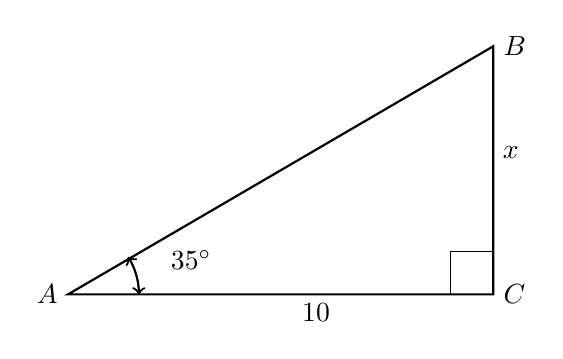
\begin{tikzpicture}[scale=0.9]
      \draw [thick]
      (0,0)node[left]{$A$}--
      (6,0)node[ right]{$C$}--
      (6,3.5)node[right]{$B$}--cycle;
      \draw (6,0)++(-0.6,0)--++(0,0.6)--+(0.6,0);
      \draw [thick, <->] (0:1) arc (0:32:1);
      \node at (20:1.4)[right]{$35^\circ$};
      \node at (3.5,0)[below]{$10$};
      \node at (6,2)[right]{$x$};
    \end{tikzpicture}
    \end{center}
    Use Graspable Math and the tangent function:
      $\displaystyle \tan 35^\circ = \frac{x}{10}$
    %https://graspablemath.com/canvas?load=_4aa5e9324049442c
    
\newpage
\item Right $\triangle ABC$ is drawn in \emph{standard position} with vertex $A$ on the origin and right $\angle C$ on the $x$-axis, as shown.
\begin{multicols}{2}
  \raggedcolumns
\begin{enumerate}
  \item Find the slope of the line segment $\overline{AB}$. \vspace{2cm}
  \item Find the measure of $\angle A$. \vspace{2cm}
  \item Find the length of the hypotenuse $AB$ using the Pythagorean Theorem $a^2 + b^2 = c^2$. (leave as a radical)
\end{enumerate}
  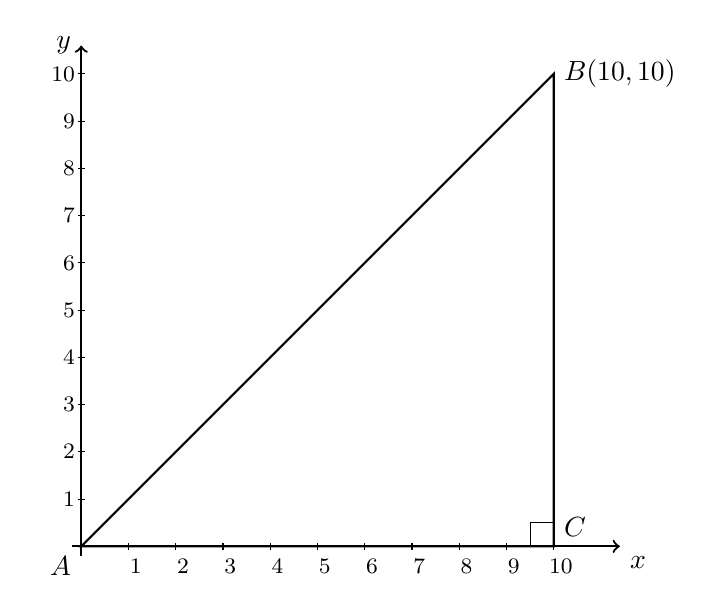
\begin{tikzpicture}[scale=0.6]
    %\draw [help lines] (-1.15,-1.2) grid (11,10);
    \draw [thick, ->] (-0.2,0) -- (11.4,0) node [below right] {$x$};
    \foreach \x in {1,2,...,10}
      \draw[shift={(\x,0)},color=black] (0pt,2pt) -- (0pt,-2pt) node[below] {\footnotesize \; $\x$};
    \draw [thick, ->] (0,-0.2)--(0,10.6) node [left] {$y$};
    \foreach \y in {1,2,...,10}
      \draw[shift={(0,\y)},color=black] (-2pt,0pt) -- (2pt,0pt) node[left] {\footnotesize \; $\y$};
    \draw [-, thick] (0,0) node[below left] {$A$}
    --(10,0) node[above right] {$C$}
    --(10,10)node[right] {$B (10,10)$}--cycle;
    \draw (10,0)++ (-0.5,0)-- +(0,0.5)-- +(0.5,0.5);
    %\draw [<->, thick] (-0.6,4.3)--(5,8.5);
  \end{tikzpicture}
\end{multicols}
%https://graspablemath.com/canvas?load=_9894332864479386

  %https://graspablemath.com/canvas?load=_024bda2a5587c074

\newpage
\item The following diagram shows a pole BT 1.6 m tall on the roof of a vertical building. \\[0.25cm]
  The angle of elevation of the top of the building from A is  
  $25^\circ$ and the distance from point $A$ to the building is 40 feet. (not drawn to scale)
    \begin{center}
      \begin{tikzpicture}[scale=0.4]
        %\draw [-, thick] (0,0)--(35:23);
        \draw [-, thick] (-4,0)--
        (0,0)--
          (17,0)--
          (22,0)--
          (22,10)--(17,10) node[left]{$B$};
        \draw [-, thick] (17,0)--(17,12)node[left]{$T$};
        \draw [fill] (0,0) circle [radius=0.1] node[below]{$A$};
        \draw [dashed] (0,0)--(17,10);
        \node at (3, 0)[above]{$25^\circ$};
        \node at (-3, 0)[below]{ground};
        \node at (19.5, 5)[above]{building};
      \end{tikzpicture}
      \end{center}
      Find the height of the building to the \emph{nearest foot}.

\end{enumerate}
\end{document}